% Figure 1
\ffigbox[\FBwidth]{
\caption{\centering Graphe \(G\)}\label{Fig:td_2_ex_12_a}
}{
    \fbox{
        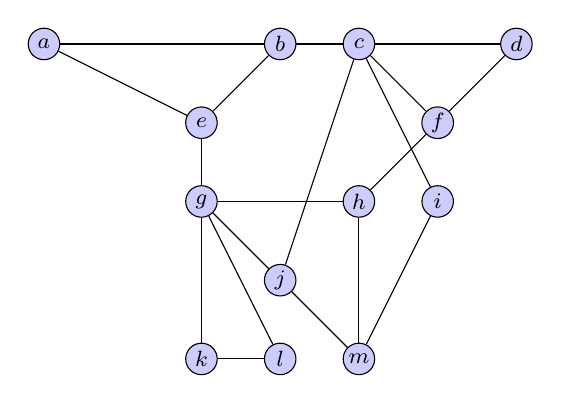
\begin{tikzpicture}[scale=1, every node/.style={circle, draw, fill=blue!20, inner sep=1pt, font=\footnotesize, minimum size=4mm}]
            \node (a) at (-2, 2) {\(a\)};
            \node (b) at (1, 2) {\(b\)};
            \node (c) at (2, 2) {\(c\)};
            \node (d) at (4, 2) {\(d\)};
            \node (e) at (0, 1) {\(e\)};
            \node (f) at (3, 1) {\(f\)};
            \node (g) at (0, 0) {\(g\)};
            \node (h) at (2, 0) {\(h\)};
            \node (i) at (3, 0) {\(i\)};
            \node (j) at (1, -1) {\(j\)};
            \node (k) at (0, -2) {\(k\)};
            \node (l) at (1, -2) {\(l\)};
            \node (m) at (2, -2) {\(m\)};


            \draw (a) -- (b);
            \draw (a) -- (e);

            \draw (b) -- (c);
            \draw (b) -- (e);
            
            \draw (e) -- (g);

            \draw (c) -- (j);
            \draw (c) -- (i);
            \draw (c) -- (f);
            \draw (c) -- (d);

            \draw (g) -- (k);
            \draw (g) -- (j);
            \draw (g) -- (h);
            \draw (g) -- (l);

            \draw (j) -- (m);
            
            \draw (i) -- (m);

            \draw (f) -- (h);
            \draw (f) -- (d);

            \draw (k) -- (l);

            \draw (h) -- (m);
        \end{tikzpicture}
    }
}